%%%%%%%%%%%%%%%%%%%%%%%%%%%%%%%%%%%%%%%%%
% kaobook
% LaTeX Template
% Version 1.2 (4/1/2020)
%
% This template originates from:
% https://www.LaTeXTemplates.com
%
% For the latest template development version and to make contributions:
% https://github.com/fmarotta/kaobook
%
% Authors:
% Federico Marotta (federicomarotta@mail.com)
% Based on the doctoral thesis of Ken Arroyo Ohori (https://3d.bk.tudelft.nl/ken/en)
% and on the Tufte-LaTeX class.
% Modified for LaTeX Templates by Vel (vel@latextemplates.com)
%
% License:
% CC0 1.0 Universal (see included MANIFEST.md file)
%
%%%%%%%%%%%%%%%%%%%%%%%%%%%%%%%%%%%%%%%%%

%----------------------------------------------------------------------------------------
%	PACKAGES AND OTHER DOCUMENT CONFIGURATIONS
%----------------------------------------------------------------------------------------

\documentclass[
	fontsize=10pt, % Base font size
	twoside=false, % Use different layouts for even and odd pages (in particular, if twoside=true, the margin column will be always on the outside)
	%open=any, % If twoside=true, uncomment this to force new chapters to start on any page, not only on right (odd) pages
	%chapterprefix=true, % Uncomment to use the word "Chapter" before chapter numbers everywhere they appear
	%chapterentrydots=true, % Uncomment to output dots from the chapter name to the page number in the table of contents
	numbers=noenddot, % Comment to output dots after chapter numbers; the most common values for this option are: enddot, noenddot and auto (see the KOMAScript documentation for an in-depth explanation)
	%draft=true, % If uncommented, rulers will be added in the header and footer
	%overfullrule=true, % If uncommented, overly long lines will be marked by a black box; useful for correcting spacing problems
]{kaobook}

% Set the language
\usepackage[english]{babel} % Load characters and hyphenation
\usepackage[english=british]{csquotes} % English quotes

% Load packages for testing
\usepackage{blindtext}
%\usepackage{showframe} % Uncomment to show boxes around the text area, margin, header and footer
%\usepackage{showlabels} % Uncomment to output the content of \label commands to the document where they are used

% Load the bibliography package
\usepackage{styles/kaobiblio}
\addbibresource{main.bib} % Bibliography file

% Load mathematical packages for theorems and related environments. NOTE: choose only one between 'mdftheorems' and 'plaintheorems'.
\usepackage{styles/mdftheorems}
%\usepackage{styles/plaintheorems}

\graphicspath{{examples/documentation/images/}{images/}} % Paths in which to look for images

\makeindex[columns=3, title=Alphabetical Index, intoc] % Make LaTeX produce the files required to compile the index

\makeglossaries % Make LaTeX produce the files required to compile the glossary

\makenomenclature % Make LaTeX produce the files required to compile the nomenclature

% Reset sidenote counter at chapters
%\counterwithin*{sidenote}{chapter}

%----------------------------------------------------------------------------------------

\begin{document}

%----------------------------------------------------------------------------------------
%	BOOK INFORMATION
%----------------------------------------------------------------------------------------

%\titlehead{The \texttt{kaobook} class}
%\subject{Use this document as a template}

\title[The Project Documentation Management]{The Project Documentation Management}
\subtitle{Methods and best pratice for a structured redaction and reuse of the project documentation}

\author[Luc Dumont]{Luc Dumont \thanks{A \LaTeX\ beginer}}

\date{\today}

\publishers{Naept Editions}

%----------------------------------------------------------------------------------------

\frontmatter % Denotes the start of the pre-document content, uses roman numerals

%----------------------------------------------------------------------------------------
%	OPENING PAGE
%----------------------------------------------------------------------------------------

%\makeatletter
%\extratitle{
%	% In the title page, the title is vspaced by 9.5\baselineskip
%	\vspace*{9\baselineskip}
%	\vspace*{\parskip}
%	\begin{center}
%		% In the title page, \huge is set after the komafont for title
%		\usekomafont{title}\huge\@title
%	\end{center}
%}
%\makeatother

%----------------------------------------------------------------------------------------
%	COPYRIGHT PAGE
%----------------------------------------------------------------------------------------

\makeatletter
\uppertitleback{\@titlehead} % Header

\lowertitleback{
	\textbf{Disclaimer}\\
	You can edit this page to suit your needs. For instance, here we have a no copyright statement, a colophon and some other information. This page is based on the corresponding page of Ken Arroyo Ohori's thesis, with minimal changes.
	
	\medskip
	
	\textbf{No copyright}\\
	\cczero\ This book is released into the public domain using the CC0 code. To the extent possible under law, I waive all copyright and related or neighbouring rights to this work.
	
	To view a copy of the CC0 code, visit: \\\url{http://creativecommons.org/publicdomain/zero/1.0/}
	
	\medskip
	
	\textbf{Colophon} \\
	This document was typeset with the help of \href{https://sourceforge.net/projects/koma-script/}{\KOMAScript} and \href{https://www.latex-project.org/}{\LaTeX} using the \href{https://github.com/fmarotta/kaobook/}{kaobook} class.
	
	The source code of this book is available at:\\\url{https://github.com/fmarotta/kaobook}
	
	(You are welcome to contribute!)
	
	\medskip
	
	\textbf{Publisher} \\
	First printed in May 2019 by \@publishers
}
\makeatother

%----------------------------------------------------------------------------------------
%	DEDICATION
%----------------------------------------------------------------------------------------

\dedication{
	The harmony of the world is made manifest in Form and Number, and the heart and soul and all the poetry of Natural Philosophy are embodied in the concept of mathematical beauty.\\
	\flushright -- D'Arcy Wentworth Thompson
}

%----------------------------------------------------------------------------------------
%	OUTPUT TITLE PAGE AND PREVIOUS
%----------------------------------------------------------------------------------------

% Note that \maketitle outputs the pages before here

% If twoside=false, \uppertitleback and \lowertitleback are not printed
% To overcome this issue, we set twoside=semi just before printing the title pages, and set it back to false just after the title pages
\KOMAoptions{twoside=semi}
\maketitle
\KOMAoptions{twoside=false}

%----------------------------------------------------------------------------------------
%	PREFACE
%----------------------------------------------------------------------------------------

%\chapter*{Preface}
\addcontentsline{toc}{chapter}{Preface} % Add the preface to the table of contents as a chapter

I am of the opinion that every \LaTeX\xspace geek, at least once during 
his life, feels the need to create his or her own class: this is what 
happened to me and here is the result, which, however, should be seen as 
a work still in progress. Actually, this class is not completely 
original, but it is a blend of all the best ideas that I have found in a 
number of guides, tutorials, blogs and tex.stackexchange.com posts. In 
particular, the main ideas come from two sources:

\begin{itemize}
	\item \href{https://3d.bk.tudelft.nl/ken/en/}{Ken Arroyo Ohori}'s 
	\href{https://3d.bk.tudelft.nl/ken/en/nl/ken/en/2016/04/17/a-1.5-column-layout-in-latex.html}{Doctoral 
	Thesis}, which served, with the author's permission, as a backbone 
	for the implementation of this class;
	\item The 
		\href{https://github.com/Tufte-LaTeX/tufte-latex}{Tufte-Latex 
			Class}, which was a model for the style.
\end{itemize}

The first chapter of this book is introductive and covers the most 
essential features of the class. Next, there is a bunch of chapters 
devoted to all the commands and environments that you may use in writing 
a book; in particular, it will be explained how to add notes, figures 
and tables, and references. The second part deals with the page layout 
and design, as well as additional features like coloured boxes and 
theorem environments.

I started writing this class as an experiment, and as such it should be 
regarded. Since it has always been indended for my personal use, it may 
not be perfect but I find it quite satisfactory for the use I want to 
make of it. I share this work in the hope that someone might find here 
the inspiration for writing his or her own class.

\begin{flushright}
	\textit{Federico Marotta}
\end{flushright}


%----------------------------------------------------------------------------------------
%	TABLE OF CONTENTS & LIST OF FIGURES/TABLES
%----------------------------------------------------------------------------------------

\begingroup % Local scope for the following commands

% Define the style for the TOC, LOF, and LOT
%\setstretch{1} % Uncomment to modify line spacing in the ToC
%\hypersetup{linkcolor=blue} % Uncomment to set the colour of links in the ToC
\setlength{\textheight}{23cm} % Manually adjust the height of the ToC pages

% Turn on compatibility mode for the etoc package
\etocstandarddisplaystyle % "toc display" as if etoc was not loaded
\etocstandardlines % toc lines as if etoc was not loaded

\tableofcontents % Output the table of contents

\listoffigures % Output the list of figures

% Comment both of the following lines to have the LOF and the LOT on different pages
\let\cleardoublepage\bigskip
\let\clearpage\bigskip

\listoftables % Output the list of tables

\endgroup

%----------------------------------------------------------------------------------------
%	MAIN BODY
%----------------------------------------------------------------------------------------

\mainmatter % Denotes the start of the main document content, resets page numbering and uses arabic numbers
\setchapterstyle{kao} % Choose the default chapter heading style

%\setchapterpreamble[u]{\margintoc}
\chapter{Introduction}
\labch{intro}

\section{The Main Ideas}

Many modern printed textbooks have adopted a layout with prominent 
margins where small figures, tables, remarks and just about everything 
else can be displayed. Arguably, this layout helps to organise the 
	discussion by separating the main text from the ancillary material, 
	which at the same time is very close to the point in the text where 
	it is referenced.

This document does not aim to be an apology of wide margins, for there 
are many better suited authors for this task; the purpose of all these 
words is just to fill the space so that the reader can see how a book 
written with the kaobook class looks like. Meanwhile, I shall also try 
to illustrate the features of the class.

The main ideas behind kaobook come from this 
\href{https://3d.bk.tudelft.nl/ken/en/2016/04/17/a-1.5-column-layout-in-latex.html}{blog 
	post}, and actually the name of the class is dedicated to the author 
of the post, Ken Arroyo Ohori, which has kindly allowed me to create a 
class based on his thesis. Therefore, if you want to know more reasons 
to prefer a 1.5-column layout for your books, be sure to read his blog 
post.

Another source of inspiration, as you may have noticed, is the 
\href{https://github.com/Tufte-LaTeX/tufte-latex}{Tufte-Latex Class}. 
The fact that the design is similar is due to the fact that it is very 
difficult to improve something wich is already so good. However, I like 
to think that this class is more flexible than Tufte-Latex. For 
instance, I have tried to use only standard packages and to implement as 
little as possible from scratch;\sidenote{This also means that 
understanding and contributing to the class development is made easier. 
Indeed, many things still need to be improved, so if you are interested, 
check out the repository on github!} therefore, it should be pretty easy 
to customise anything, provided that you read the documentation of the 
package that provides that feature.

In this book I shall illustrate the main features of the class and 
provide information about how to use and change things. Let us get 
started.

\section{What This Class Does}
\labsec{does}

The \Class{kaobook} class focuses more about the document structure than 
about the style. Indeed, it is a well-known \LaTeX\xspace principle that 
structure and style should be separated as much as possible (see also 
\vrefsec{doesnot}). This means that this class will only provide 
commands, environments and in general, the opportunity to do things, 
which the user may or may not use. Actually, some stylistic matters are 
embedded in the class, but the user is able to customise them with ease.

The main features are the following:

\begin{description}
	\item[Page Layout] The text width is reduced to improve readability 
	and make space for the margins, where any sort of elements can be 
	displayed.
	\item[Chapter Headings] As opposed to Tufte-Latex, we provide a 
	variety of chapter headings among which to choose; examples will be 
	seen in later chapters.
	\item[Page Headers] They span the whole page, margins included, and, 
	in twoside mode, display alternatively the chapter and the section 
	name.\sidenote[][-2mm]{This is another departure from Tufte's 
	design.}
	\item[Matters] The commands \Command{frontmatter}, 
	\Command{mainmatter} and \Command{backmatter} have been redefined in 
	order to have automatically wide margins in the main matter, and 
	narrow margins in the front and back matters. However, the page 
	style can be changed at any moment, even in the middle of the 
	document.
	\item[Margin text] We provide commands \Command{sidenote} and 
	\Command{marginnote} to put text in the 
	margins.\sidenote[][-2mm]{Sidenotes (like this!) are numbered while 
	marginnotes are not}
	\item[Margin figs/tabs] A couple of useful environments is 
	\Environment{marginfigure} and \Environment{margintable}, which, not 
	surprisingly, allow you to put figures and tables in the margins 
	(\cfr \reffig{marginmonalisa}).
	\item[Margin toc] Finally, since we have wide margins, why don't add 
	a little table of contents in them? See \Command{margintoc} for 
	that.
	\item[Hyperref] \Package{hyperref} is loaded and by default we try 
	to add bookmarks in a sensible way; in particular, the bookmarks 
	levels are automatically reset at \Command{appendix} and 
	\Command{backmatter}. Moreover, we also provide a small package to 
	ease the hyperreferencing of other parts of the text.
	\item[Bibliography] We want the reader to be able to know what has 
	been cited without having to go to the end of the document every 
	time, so citations go in the margins as well as at the end, as in 
	Tufte-Latex. Unlike that class, however, you are free to customise 
	the citations as you wish.
\end{description}

\begin{marginfigure}[-5.5cm]
	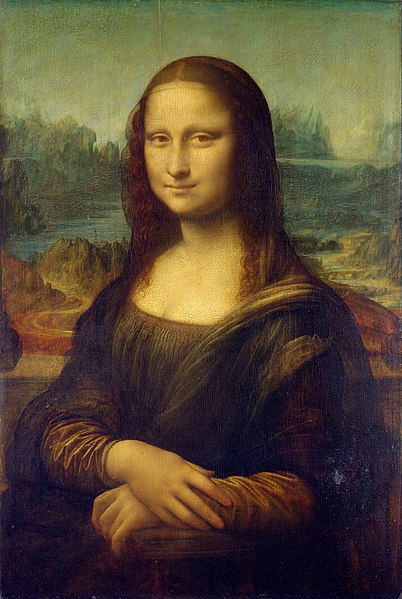
\includegraphics{monalisa}
	\caption[The Mona Lisa]{The Mona Lisa.\\ 
	\url{https://commons.wikimedia.org/wiki/File:Mona_Lisa,_by_Leonardo_da_Vinci,_from_C2RMF_retouched.jpg}}
	\labfig{marginmonalisa}
\end{marginfigure}

The order of the title pages, table of contents and preface can be 
easily changed, as in any \LaTeX\ document. In addition, the class is 
based on \KOMAScript's \Class{scrbook}, therefore it inherits all the 
goodies of that.

\section{What This Class Does Not Do}
\labsec{doesnot}

As anticipated, further customisation of the book is left to the user. 
Indeed, every book may have sidenotes, margin figures and so on, but 
each book will have its own fonts, toc style, special environments and 
so on. For this reason, in addition to the class, we provide only 
sensible defaults, but if these features are not needed, they can be 
left out. These special packages are located in the \Path{style} 
directory, which is organised as follows:

\begin{description}
	\item[kao.sty] This package contains the most important definitions 
	of macros and specifications of page layout. It is the heart of the 
	\Class{kaobook}.
	\item[kaobiblio.sty] Contains commands to add citations and 
	customise the bibliography.
	\item[packages.sty] Loads additional packages to decorate the 
	writing with special contents (for instance, the \Package{listing} 
	package is loaded here as it is not required in every book). There 
	are also defined some useful commands to print the same words always 
	in the same way, \eg latin words in italics or \Package{packages} in 
	verbatim.
	\item[kaorefs.sty] Some useful commands to manage labeling and 
	referencing, again to ensure that the same elements are referenced 
	always in a consistent way.
	\item[environments.sty] Provides special environments, like boxes. 
	Both simple and complex environments are available; by complex we 
	mean that they are endowed with a counter, floating and can be put 
	in a special table of contents.\sidenote[][-2mm]{See 
	\vrefch{mathematics} for some examples.}
	\item[theorems.sty] The style of mathematical environments. 
	Acutally, there are two such packages: one is for plain theorems, 
	\ie the theorems are printed in plain text; the other uses 
	\Package{mdframed} to draw a box around theorems. You can plug the 
	most appropriate style into its document.
\end{description}

\marginnote[2mm]{The audacious users might feel tempted to edit some of 
these packages. I'd be immensely happy if they sent me examples of what 
they have been able to do!}

In the rest of the book, I shall assume that the reader is not a novice 
in the use of \LaTeX, and refer to the documentation of the packages 
used in this class for things that are already explained there. 
Moreover, I assume that the reader is willing to make minor edits to the 
provided packages for styles, environments and commands, if he or she 
does not like the default settings.

\section{How to Use This Class}

Either if you are using the template from 
\href{https://latextemplates.org/template/kaobook}{latextemplates}, or if 
you cloned the GitHub 
\href{https://www.github.com/fmarotta/kaobook}{repository}, there are 
infinite ways to use the \Class{kaobook} class in practice. To get started,
find the \Path{main.tex} file which I used to write this book, and edit it; this 
will probably involve a lot of text-deleting, copying-and-pasting, and rewriting.

To compile the document, assuming that its name is \Path{main.tex}, you 
will have to run the following sequence of commands:

\begin{lstlisting}[style=kaolstplain,linewidth=1.5\textwidth]
pdflatex main # Compile template
makeindex main.nlo -s nomencl.ist -o main.nls # Compile nomenclature
makeindex main # Compile index
biber main # Compile bibliography
makeglossaries main # Compile glossary
pdflatex main # Compile template again
pdflatex main # Compile template again
\end{lstlisting}

You may need to compile the template some more times in order for some 
errors to disappear. For any support requests, please ask a question on 
\url{tex.stackexchange.org} with the tag \enquote{kaobook}, open an 
issue on GitHub, or contact the author via e-mail.


\pagelayout{wide} % No margins
\addpart{Stakes and issues}
\pagelayout{margin} % Restore margins

\setchapterpreamble[u]{\margintoc}
\chapter{Why writing project documentation is boring?}

“We’ll have to do documentation again ? Really !”

We hear this a lot when we tell a teammate he will have to write some documentation for the project. We are engineers and we have had to deliver many many documents. So let’s be honest, documentation is boring. But when it is well done, it is a very valuable asset. It allows to make once mind, settle the project, detail, save, index and share ideas and innovative solutions (God bless Ctrl+F). Documentation would be so much less painful if it wasn’t for some productivity traps that are so time consuming and generate pressure. Fortunately they can be avoided …

Here is a non exhaustive list of what is unpleasant when writing a document, and how to overcome it.

\section{Writing about a topic we do not master}
There is often only one person dedicated to write all the documentation of a project. It avoids to manage a planing for several editors. Besides the final product will have one consistent tone. But this one person may not master all the different fields of technology taking part in the project to give a complete description of them. This situation has been encountered by a person we met.

\begin{kaobox}[frametitle=A former teammate engineer destimonial]
	I had been asked to write the tests to do on a product to ensure it meets our customer needs. It was a complex task because I was completely unfamiliar with one of the involved technologies. I had to ask to the expert and I worked hard to understand how it was working to finally write some relevant tests. It took me several iterations of them but it ended up working. I up skilled a lot on this technology but we may had lost some time and I got some cold sweats.
\end{kaobox}

Giving someone a task he isn’t skilled enough to perform without some learning can lead to an unsecured mindset. But sometimes, by lack of available experts, we cannot do otherwise.

Today there are more and more collaborative softwares easing the teamwork (you can share a document and comment it in real time with Microsoft Word or Google Docs for example). We have met lots of companies making their own tutorial videos to share some specific knowledge between collaborators. Besides, the “reuse”, which means starting from previous documents to write the new ones, is becoming the rule. It is always easier to update a previous revision and adapt it to the new project, than starting the document from scratch.

\section{The WYSIWYG editors}
WYSIWYG stands for: “What You See Is What You Get”. It means what you see on screen is its real rendering. This is how works the main text editors like Microsoft Word. This makes those softwares very intuitive and easy to use. Everybody knows how to write something on Word!

But when you write project documentation, you probably need to add comments, track modifications, draw tables, put some automatic fields (page numbers, etc)...

This leads the software to use lots of RAM to be able to render the final view of your document in real time with all those features. It does it seamlessly for a short file. But your computer might start to sweat when your document reaches the hundred of pages. Then the text editor reactivity is getting slower and can finally crash (true story)!

\LaTeX{}

To avoid hitting the save button every minutes, there are text editors with different philosophy. LaTeX is one of those and it is free. But it requires some learning first. Its way to do is to differentiate the content from the document layout in different files. On one side you write your text with tags in it. Those tags will indicate where you want the graphical features such as a figure, a table, a title, etc. On the other side. At this moment your text doesn't look like the final rendering at all ! On a second file you configure the display of those graphical features. Finally you run LaTeX on those files and it builds your document. You may have to run several times LaTeX with different settings to get the exact document you had in mind. But then you will never have to correct the layout. It will never change because of a text modification. Content and layout do not interfere.

Ok, I confess it seams a little more touchy than Word. But you should give it a try because it is so much more powerful and rather easy to master !
Fortunately the WYSIWYG text editors get auto-save feature that are more and more effective.


\section{Validation workflows}
Usually every document shall be delivered to the customer. To ensure the document reaches the quality standard of the company, it must be checked by several reviewers through a validation workflow.

But the reviewers expectations may vary if they don’t know the project with the same level of details. So a simple document review can turn into an argumentation about the project itself. Here we go again, those reviews must be planed:

\begin{enumerate}
	\item Select reviewers for the project and stick with them all along. You can assign them to specific parts of the document corresponding to there expertise.
	\item Schedule the reviews in a finite period of time.
	\item Collect their remarks in one place, like a spreadsheet for example. This will ease their management en then the document update.
\end{enumerate}


\section{The level of detail}
Whatever the product, its specifications can be two pages long or one hundred. The difference lays in the level of details.

There is no miracle spec. They can be very light, it is cheap but you risk to put the project on hold with non-anticipated issues. They can be very detailed and plan everything but not only they are very expensive but every review will be very long.

So you have to meet halfway. A good practice is to make a first iteration allowing someone who doesn’t know the project to understand it and start working on it. Then, very regularly, with small steps, update the document throughout the project. Be careful not to overkill the quality, it is not a piece of art, it is a tool. Documentation must not drain you effort over more critical activities.


\section{The lack of interest}
Some documents have no other purpose than being archived. They are just new entries to some dead database and will never be referred back to ever again. They are artifacts from an obsolete but persistent workflow. The french philosopher Julia de Funes says that loss of meaning happens when the purpose disappears in favor of its mean.

It is time to question this workflow because those documents have a cost (an not only a financial cost). What impact on the collaborator mindset will have this lack of interest for his work?

On the other hand, such a documentation can be highly valuable! It can be a precious asset to kickstart similar new projects. If they are just saved and correctly indexed in a database (like Sharepoint), a simple request on its search engine will rapidly identify the most relevant documentation to reuse. And by constantly updating this database, the company not only saves but grows its knowledge, its expertise. It turns this previously frozen load into a living strategic asset. The author becomes aware that he is building knowledge other will trust and use. It is a far more gratifying activity!

\section{Working blind}
The blank page syndrome is not a novelist privilege. Being in charge of a complex specification document can be petrifying if we don’t know where to start. Should I start by this element or this one ? Haven’t I forgot anything ? Is it precise enough ? It is really clear ? Should I explain this or is it obvious?

It is always a good move to start from something known and verified. We take a previous document, we drop what is out of context, we keep the frame and what is reusable and we start from here. The old parts will help us, guide us to be more exhaustive about the new project.

The next step is to build templates with pre-filled sections. It avoids us to rewrite over and over the same elements in all documents. Those templates can have entitled sections for every possible aspect of the projects. All of them will rarely be filled but they help ensure we forgot nothing. Project after project, those templates are updated and the document quality rises up.

The website FYI presents a very large amount of templates and dashboards for every productivity tools to Getting Work Done! (their moto)

\section{Conclusion}
After all, we see that documentation might not be a problem at all. Organization, effective management and methodology can easily turn what was a painful activity into a real engine for productivity and motivation!


\setchapterpreamble[u]{\margintoc}
\chapter{Why writing documentation is boring}
\label{sec:WhyBoring}

Writing a specification document can feel ea“We’ll have to do documentation again ? Really !”

If only that could be so easy. Sometimes it is. But usually not. We will go through 4 major difficulties in this process from a simple McDonald’s order to a wedding planning! 

12:15 AM in a McDonald’s fast-food:\\
– Hello, I’d like a Big Mac, a Coke and a large portion of fries please.\\
2 minutes later :\\
– Here is your order, have a nice day.\\
– Thank you, goodbye.

8:30 PM in a fancy restaurant:\\
– Honey, will you marry me ?– Yes !!!\\
One year later, 2 weeks before wedding:\\
– Great Scott! Nothing is going well! The whole table disposition from the wedding planer has to be remade : Anthony cannot bear his brother and my cousins have canceled. All the tablecloths are taupe but they should be beige. We totally forgot to organize the brunch. And you remember your Mexican music band? Wee cannot afford it!!!

\begin{kaobox}[frametitle=Disclaimer]
	This article isn’t in any way a celebration of the well-know fast food license. But it is a very good example of how a customer experience can be fully optimized
\end{kaobox}

Either for a project as quick as a fast food order, or for one as ambitious asa wedding planning, the first step is always the same. We list all that we want and give it to some professionals who will take care of everything.In both cases, we identified 4 characteristics that are very important to master if we want the most seamless communication possible. Let’s dive into them.


\section{The context}

In the McDonald’s order placement scenario, the context issue is solved by your presence into the restaurant. If, by any odd circumstance, you would order a burger in a shoe shop for example you would get a good laugh from the seller or maybe a suspicious look.

In the wedding case, we observe that we haven’t explain enough of the family situation to the wedding planer: the enemies brothers and the not so reliable cousins.

It is very important to give the most complete context for a project to our supplier, to detail our activity. Like that, even before entering the core of your need, he will be able to tell if he is qualified enough for the job or not. To do so, you can present:

\begin{itemize}
	\item Your company, its activities, some technical concepts you need your supplier to understand
	\item Your market and your customers
	\item The project your need is about
\end{itemize}


\section{The vocabulary}
At McDonald’s, the vocabulary to order a menu is clearly defined thanks to the panels above the cashiers. They show all the burgers and side dishes available. Their combinations are rather finite and the customers have all the time to build their order while they wait in line.

For wedding, we can have very precise expectations, like beige tablecloths for example. But if we haven’t correctly defined with the planer what we have in mind when we talk about the beige color, we can end up with taupe!

So clearly stating the vocabulary is essential. There is a probability that you will employ the same wording but with a slightly different meaning. That difference can generate big consequences on the budget or the planning by the end of the project before you understand why.

A simple glossary of the most important elements, placed in the opening of the document, can ensure all the stakeholders that they speak the same language. Do not hesitate to update it during the project in any doubt appears.


\section{The maturity}
This is the most common characteristic in the fast food orders: how many customer arrive at the cashier and are still building up their order. But it’s in the name: fast food! If the order isn’t complete, it won’t take the customer too much time to come back with a new order.

Maybe the Mexican band wasn’t necessary for an already beautiful wedding. Or at least, it wasn’t totally affordable. It would probably be wiser to abandon this “requirement” to secure the event.

More seriously, it is difficult to precisely estimate the maturity of a project at the beginning. Is this item relevant? Useful? Is it a “must have” or a “nice to have”? Do we really need a hammer to kill a fly? Or a rolled newspaper is enough? We can employ the 5 why technique: questioning a need 5 times in a row to find out its root, its prime cause.
We can also openly talk about it with our supplier and give him the opportunity to make suggestions, and for us to trust its expertise.


\section{The exhaustiveness}
We are always asked if we want anything more in a fast food. It is to drive us to buy more? It is to be sure we, the customers, are always pleased? I will leave you to this mystery. But this question has the benefit to ensure an higher maturity, completeness of our order, avoiding us to come back for something we would have forgotten.

Oh, oh, oh! We totally forgot to think about the brunch for the day after! We need a whole new budget for it and talk about it with the caterer! This wedding planner is very lame. He should have warned us.

This issue goes hand to hand with the maturity of our needs. Exhaustiveness asks us “Did you think of it all? Have you not forgot something?” Very hard to tell in advance.
To secure those risks and avoid any “holes in the racket” (we say “trou dans la raquette” when something is missing), we can check what we did in previous projects. We can consult their documentation and use it like a starting checklist. Some parts could be completely reusable and some other may need minor updates. In the same mindset, we can build templates for the projects: pre-filled documents with commonly used chapters and checklists. Some will be abandoned, some will be kept, augmented, optimized

Once again, we can brainstorm with our supplier and summon his expertise. His fresh look upon the project can enlighten some dark areas.


\pagelayout{wide} % No margins
\addpart{Tools}
\pagelayout{margin} % Restore margins

\setchapterpreamble[u]{\margintoc}
\chapter{Needs assessment : some good practices}
\label{sec:NeedAssessement}
When we write a needs assessment or a specification document for a supplier, we try to be as complete as possible. The document turns into a list of expected features. Here are some good practices to build the most efficient request.

\section{Sorting the requirements by themes}
The more requirement we have, the more difficult it will be to get the big picture. So we have to sort them by their subject, by the technology they are about, or by the expertise they require.

For example, to specify a bike, we gather as follow:
\begin{itemize}
    \item All the requirements about the wheels
    \item All the requirements about the brake system
    \item All the requirements about the gear management
    \item \dots
\end{itemize}

Therefore the supplier will easily be able to choose his best qualified experts for the job. The needs assessment document can now be shared with all of them, and each of them can take on the part about his field of expertise.

\section{The shorter, the better}
When writing a needs assessment, we may intend to write long descriptions for several reasons:

\begin{itemize}
    \item we are in a train of thoughts
    \item we describe several connected elements
    \item the subject is complex and requires lots of details
\end{itemize}

But the problem happens when the customer brings an evolution to its initial assessment. We have to find out what are the impacts on our features specifications. Without an accurate indexing of the requirement and a clear view of their content, we will have to read the whole document again. That can take a lot of time.

But if, from the beginning, we have tried to write the shortest possible requirements, each of them deals only with a specific point, it will increase their quantity but it will also strongly optimizes the following:

Their \textbf{indexing}: one requirement describes one limited subject.

The easiness of their \textbf{update}: we know at one glance if the requirement must be updated because of an evolution.

Their \textbf{traceability}: it is way easier to link the need to the feature.

Their \textbf{testing}: the shorter the requirement, the easier to prove that the final product matches it.

Their \textbf{reusability}: in a future project, if the client defines a similar need, it will be very easy to reuse the requirements from a previous project. You may have to perform some adaptations but they will be limited. Just like a piece of Lego you can reuse in a new construction.

\section{A needs assessment requirement must describe a need, not a feature}
When we write a needs assessment, the purpose is to subcontract the product development to a supplier. We do so because we do not have the resources or the knowledge to do it ourselves.

But if we have a very detailed idea of what we want, we may be tempted to write a full feature specification. Which is a totally different document and we advise you to agree with your supplier about it. Unless, be careful not to give too much specific details and force your supplier. By giving him to much technical details, you won’t summon the expertise you were asking in the first place by hiring him. It is risky for the project to mix your need and the solution specification in the same document :

\begin{itemize}
    \item Are you sure the features you have in mind will match your needs? (Have you ever heard about the XY problem?)
    \item Your feature solutions, are they all compliant?
    \item What are you expecting from your supplier? An expertise or just some manpower?
    \item What about its added value?
    \item What about its responsibility?
\end{itemize}

That’s why it is important to distinguish your needs from the final product features.

\section{Using "shall"}
English language is very generous on how to express what we want. Some of the manners can be ambiguous and may compromise the message we want to deliver.

\begin{itemize}
    \item “I would like“, “I wish“… Is this a strong order or the expression of a nice to have?
    \item “I want“… Is it a personal request? Is it part of the contract?
    \item “It has not to”… Should we understand it has a strong prohibition or the freedom not to do it ?
\end{itemize}

First of all, you can choose any verb but the most important is to choose one and stick to it during all the project. A commonly used one we recommend is to employ “shall”. It is simple, kind of binary and rather not questionable:

\begin{itemize}
    \item “XXX shall be…” or “XXX shall do…“: it describes what is expected
    \item “XXX shall not be…” or “XXX shall not do…“: it describes what must not be expected
\end{itemize}

\section{Pay attention to all the possible interpretations}
A same text can be understood differently depending on the reader’s expertise, experience, position and even his current state of mind. So there is a chance that he has a slightly different interpretation than yours. This risk must be considered seriously as it can lead to severe project shift. Do your words express your thoughts? Is there any room for a misunderstanding? Do you share with your supplier the same meaning for every concepts of the project? The road to hell is paved with good intentions.

So, before delivering a document, a simple peer review by one of your teammates will very efficiently reduce the risks of misunderstanding. And adding a glossary at the beginning of the document to define the sharpest concepts will reduce the risks even more.


\section{Is your need testable?}
Is it even possible to check that the product matches every specific requirement?

Imagine that one of your requests asks for “the fastest” car. Alright. How can your supplier ensure you that the car he delivered is “the fastest”? This is a tricky demand hardly verifiable. First of all, how fast can a car go today? What if this speed is different than the one you had in mind? Who is right?

It is much safer to build the requests with measurable elements. These won’t let any doubt about what you are expecting and will be undeniably verifiable.

“The car shall be able to reach the speed of 250 kph”. The delivered car goes up to 300 kph. Ok! It matches the need, the requirement is validated!

For more details about tests, read our article about validation plans. It is also in french, we will publish it in english soon too.


\setchapterpreamble[u]{\margintoc}
\chapter{Reading sheet, an easy tool for collaborative review}
\label{sec:ReadingSheet}

Finally ! You did it ! The document is finished. But before definitely freeze it, it has to be validated. So you send it to several people who will read it and comment it. But one week later, you have dozens of e-mail from them and 4 different corrected copies of your document. Those exchanges have brought more questions than answers. The reading sheet allows you to structure the validation process and to take every remark into account.

Depending on the size and complexity of the project, it is required to validate its documentation by one or several people:

\begin{itemize}
    \item The project manager who is responsible for the customer
    \item A peer reviewer who checks the technical content
    \item A quality expert who ensures the document matches the company’s quality criteria
    \item …
\end{itemize}

The customer who tells if the document meets his needs.
Without a clear workflow, every reviewer can comment the document in a different way:
\begin{itemize}
    \item by mail
    \item by telling you his remarks at the coffee machine
    \item within his own document copy
    \item in the MS Word comment section
    \item by hand-writing his remarks on a print
    \item …
\end{itemize}

Managing so many different channels can jeopardize the final quality of the document. How to be sure none of the remarks is lost? Is there some duplicated ones? Are they all consistent? Etc.

\section{One file to collect them all}
The reading sheet is a tool to collect all the remarks about a document (or anything else) in the same place and organize them to address them all.

This is a simple spreadsheet, an MS Excel file, in which every line is a reviewer remark. It contains several columns to fill. Those columns are indicators allowing to sort the remarks and ease their management. In the following paragraph we will detail the most commonly used columns.


\section{The columns}

Here is an example of a reading sheet based on the feedback of our own experiences and the ones of people we met.

\begin{table*}[h]
	\centering
		\begin{tabular}{|c|c|c|c|c|c|c|c|c|c|}
			\hline
			\ ID & Location & Category & Severity & Description & Reviewer & Responsible & Status & Comment & Action \\ 
			\hline
			&&&&&&&&&\\
		\end{tabular}
	\caption{Headers for a reading sheet}
	\label{tab:HeaderRS}
\end{table*}

This list isn’t exhaustive. Some of them might be useless and you might need some other depending of your process. Please share with us in the comment section those data you use in your own reading sheets.

\subsection{ID}
It is a simple but unique number, incremented for each remark. The purpose is to identify it. If a remark must be erased, its ID has to be erased too and it cannot be used for another one or it could lead to misunderstanding.

\subsection{Location}
Any remark has to be precisely located! The author must not be forced to read the whole document to find the object of the remark. It wouldn’t be very efficient.
A first way of doing this is to locate it with the document page. But it isn’t the best practice because if a section is added to the document, for example, the updated can turn to be totally irrelevent.
The ideal way is to locate the remark with the smallest paragraph title its object belongs too. Like this, it doesn’t matter if the paging changes. The author will quickly find it with the table of content.

The location shall be given by the reviewer.

\subsection{Category}
All the remarks are not from the same kind. They can be about:

\begin{itemize}
    \item a comprehension question
    \item a spelling mistake
    \item an author misunderstanding of the need
    \item etc.
\end{itemize}

Therefore remarks can be sorted by categories. It will be easier to manage them. Fro example, the author may want to fix all misspelling ones before going to the semantics.

It is important to have a limited number of categories for the sorting to be useful. But on the other hand, it is required that list to be exhaustive enough to cover any kind of remarks. Here are some possible categories:

\begin{itemize}
    \item Question
    \item Misspelling
    \item Nonsense
    \item Layout
    \item Error
\end{itemize} 
Category shall be given by the reviewer.

\subsection{Severity}
Severity is a second sorting criteria. Two remarks from the same category can have different weight. This weight can be defined by the severity.

For example, the severity scale can go from level 1 telling the remark is painless for the project, to level 5 telling the pursuit of the project is stopped as long as this remark isn’t solved.

It is really important that this severity scale is clearly defined and shared with everyone before starting the reviews.

Severity shall be given by the reviewer.

\subsection{Description}
This is the description of the remark itself. It is important this description is as detailed as possible. You can insert a short document extract to ease its understanding, highlight important words. It shall be precise enough for the author to not have any doubt about the issue.

Description shall be given by the reviewer (obviously).

\subsection{Reviewer}
If the author knows who gave each remark (several reviewer can add remarks to the reading sheet), he will know who to ask if he needs further information to solve the issue.

Reviewer shall be given by… the reviewer.

\subsection{Responsible}
Here we talk about the person in charge of solving the remark. As this person can be different for some remarks (many people may have written the document together), the person responsible must be defined for each remark.

But it is not up to the reviewer to decide who is in charge of his remark, beside he may not have a clue about who is competent for it.
If there is only one author for the document, so it’s a no-brainer: responsible = author.
If there are several authors, there must be a manager driving the team. So it is up to him to tell who is in charge of each remark.

\subsection{Status}
It simply is the status of the remark. Depending on your review workflow, this status can take several values. Here are some examples of possible values:

\begin{itemize}
    \item \textbf{Open} (set by the reviewer)\\When a new remark is added, it is “open” for resolution, meaning it shall be processed by the responsible.
    \item \textbf{Duplicated} (set by the person responsible)\\If by any chance a remark tells the same thing than another one, the responsible gives this status to it. It happens when several reviewers use the shame reading sheet to gather their remarks.
    \item \textbf{Accepted} (set by the person responsible)\\It is a temporary status. On a first hand, the responsible may have a look on all remarks at once. He may want to check for the duplicated ones or to see if all of them are relevant. When he wants to tell if a remark is relevant and he is willing the solve it, he sets this status.
    \item \textbf{Rejected} (set by the person responsible)\\But when he believes a remark is not relevant, he can set it to”Rejected”. He shall explain why it is irrelevant in the comment section. Then the reviewer will decide if he agrees.
    \item \textbf{Corrected} (set by the person responsible)\\The responsible has accepted and fixed the document according to the remark. He tells it is “Corrected” then the reviewer can check if he is OK the correction.
    \item \textbf{Closed} (set by the reviewer)\\If the correction is satisfying, the reviewer can set the remark to “Closed”. Case closed!
\end{itemize}

\subsection{Comment}
This section can be used by the responsible to bring a comment on the remark resolution. He can explain here how he corrected it.
This is where he shall explain why he eventually rejected the remark.
If the remark consisted in a simple question, this is where the answer shall be brought.

Be careful to not turn this comment section into a chatroom about the remark.

If required, the comment can be added by any stakeholder.

\subsection{Action}
Some remarks and resolutions can have a higher scope than just updating the document. They may require to update the whole project, change the contract, the planning, the budget, the product…

So one remark can have some ripple effect implying the use of a project dashboard action, a bugtracking issue (see our french article, but soon translated)… Those item have their own identification references. So you can use the Action column to quote those references and ensure the traceability of the cross-application resolution.

If required, the action shall be given by the responsible.

\section{Best practices}
\subsection{Index the reading sheet}
As soon as you create a new reading sheet, give it a unique reference. It will allow everyone to quote it in the document it talks about and ease their management if you have several of them.
\subsection{Use one for each document delivery}
Every time you send a document to someone, if this someone can comment it, join a blank reading sheet. So he can add its remarks directly into it, saving you the task to copy and past them from his e-mail.
\subsection{Traceability}
When you start to update a document with all your reviewers remarks, indicate in the document that it has evolved thanks to the reading sheet <insert its reference>. So anyone can track back the origin of those evolutions.
\subsection{Precision}
Never hesitate to give the most exhaustive description for a remark. The responsible shall have enough information to not need to call you back to remove a doubt.

Once more, the location in the document of the object of the remark shall be as precise as possible for the responsible shall not lose time finding it.

\section{Pros and cons}
\subsection{Pros}
You can build a reading sheet out of any spreadsheet editor (MS Excel, Google Docs, OpenOffice…). So that is a really easy tool available to anyone.

It is not only applicable to a document review but, actually, to any kind of reviews: source code, graphic elements, product… As soon as you need to collect remarks, the reading sheet is relevant.

Even if there are several reviewers, you can send them each a reading sheet and then gather all of them into one (you can even write a script to do it automatically). But with the today online editors, it is even easier to work on a shared document.
\subsection{Cons}
Be careful not to use a reading sheet and its comment section as a forum with an endless message chain. Comments shall just be comments. Otherwise just pick up the phone.

Obviously it is another file to manage in the project and you may already have lots of them.

You better have a big screen or even two. It is nice to have the document you are reviewing on a side and its reading sheet on the other side. Switching from one to the other on a single screen might drive you crazy.

\section{Conclusion}
The reading sheet is a very easy and versatile collaborative tool. It allows you to structure and easily manage any reviewing process. Even if more and more software come with comment features, a reading sheet is a quick and simple solution to implement with anyone regardless of having the last fancy webapp. You can find a reading sheet template for free on our Github repository.

\setchapterpreamble[u]{\margintoc}
\chapter{The traceability matrices}
\label{sec:TraceabilityMatrices}

In a customer request for proposal, the need is usually given through a list of requirements. The supplier sends back a proposal showing his solution through a list of specifications. The coverage between requirements and specifications can take different shapes:

\begin{itemize}
    \item 1 to 1: one specification covers one requirement
    \item 1 to many: several specifications are used to cover only one requirement
    \item Many to 1: several requirements are covered by one specification.
\end{itemize}

But in practice, it is rather a mix of the three leading to a maze of coverage. Fortunately the traceability matrix shows up to bring some order.


\section{Traceability, this entangled mess}
A document size can vary a lot depending on the different fields of activity it deals with. To explain this, I will take an example I know well. Consider a request for proposal (RFQ) about an aeronautic calculator. Please don’t leave yet! I’ll make it clear.

In a plane, there are dozens of calculators. Those are computers without a screen or a keyboard. They manage everything, from the air conditioning to the brakes, the doors, the electrical power distribution, etc. Whether their tasks are complex or very complex, their request for proposal can easily reach a hundred pages and hundreds of requirements. Several expertises are involved to describe all the requirements. For example:

\begin{itemize}
    \item electronics for the circuit boards
    \item mechanics for the case housing the circuit boards
    \item developers for the embedded firmware of the circuit boards
    \item etc.
\end{itemize}
Then this RFQ is sent to a supplier. He will study it with his teams to build the specifications. Sometimes several requirements can be covered by the same specification.

\subsection{Many to one}
Customer requirement 1: the circuit board shall be hermetically protected\\
Customer requirement 2: the case shall have the following measurements : X, Y, Z

Supplier specification 1: the case shall be from the brand B and the model M

Therefore the supplier specification hits two birds with one stone because the chosen case matches both the requirements.

\begin{figure}[h]
    \centering
    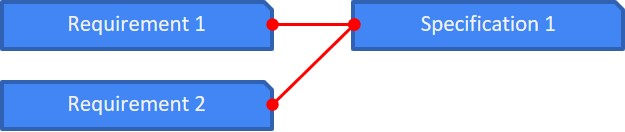
\includegraphics[]{ManyToOne.jpg}
    \caption{2 requirements covered by 1 specification}
    \label{fig:ManyToOne}
\end{figure}

\subsection{One to many}
But sometimes, it is the other way around! The requirement is so complex, it requires several specification to be fully covered:

Customer requirement 3: the circuit board shall be fully operational while the plane is flying (it’d better be).

Supplier specification 2: the electronic components of the circuit board shall be from the S series. The S series components stay operational even at temperatures below -50°C (this is the outdoor temperature at cruising altitude).

Supplier specification 3: the case shall have an S shield to protect the circuit board from electromagnetic fields.

Supplier specification 4: the case shall be mounted on suspending plot to protect the circuit board from mechanical vibrations.
\begin{figure}[h]
    \centering
    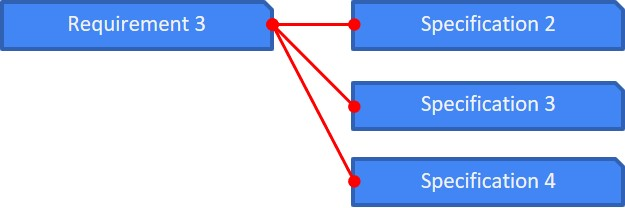
\includegraphics[]{OneToMany.jpg}
    \caption{1 requirement covered by 3 specifications}
    \label{fig:OneToMany}
\end{figure}

So we see here that the complexity of the coverage between requirements and specifications can quickly increase. Just like a spaghetti dish!

\begin{figure}[h]
    \centering
    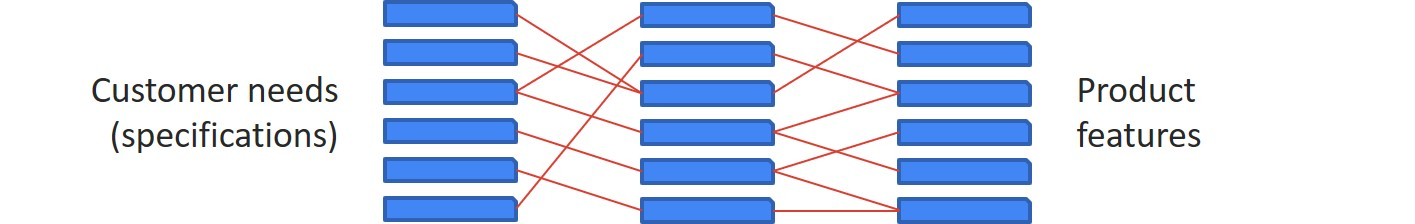
\includegraphics[]{traceability}
    \caption{Many requirements entangled to many specifications}
    \label{fig:WholeTraceability}
\end{figure}

\section{Ok but how exactly?}
\subsection{The structure}
A traceability matrix is an two-columns table where are exhaustively listed every coverage link between every requirements and every specifications. Our previous example would give the following matrix:

\begin{table*}
	\centering
		\begin{tabular}{|c|c|}
			\hline
			Customer Requirements & Supplier Specifications\\
            \hline
            Customer requirement 1 & Supplier specification 1\\
            \hline
            Customer requirement 2 & Supplier specification 1\\
            \hline
            Customer requirement 3 & Supplier specification 2\\
            &Supplier specification3\\
            &Supplier specification 4\\
            \hline
		\end{tabular}
	\caption{Downstream Traceability Matrix}
	\label{tab:DownstreamTraceabilityMatrix}
\end{table*}

On the left, there is the list of the customer’s requirements in the same order they appear in the RFQ. There are given by their title only (or their ID) to avoid an overloaded table.
On the right, for each requirement, the list of the covering customer specifications.

It is very important that on the left column, each requirement appears once and only once. The purpose here is to ensure every requirement is covered by at least one specification.
On the contrary, on the right column, we observe the supplier’s specification 1 is listed twice. This is absolutely normal as this specification matches both customer requirement 1 and customer requirement 2.

\subsection{The point of view and coverage quality}
We can say this matrix adopts the customer’s point of view. It goes from the RFQ to the specifications, that is why it is called the \textbf{Downstream Traceability Matrix}. Once completed, we know exactly the coverage of the customer need. And if one requirement as no specification match, we know the specification document isn’t complete.

But be careful as the devil always hides in the details! The traceability matrix can only tell if a requirement is covered by a specification. I cannot tell if this specification IS ENOUGH to cover the requirement.
Let’s consider again the customer requirement 3. We see it is covered by the following specifications:

\begin{itemize}
    \item Supplier specification 2
    \item Supplier specification 3
    \item Supplier specification 4
\end{itemize}

For example, if the supplier specification 4 is omitted, from the matrix point of view, the customer requirement is still covered. But in reality, without the specification 4, the product wouldn’t match the need.

\section{The other traceability matrices}
We can change the point of view of the matrix to observe the project’s traceability from another angle to ease its management.

\subsection{Upstream Traceability Matrix}
We saw the customer’s point of view with the downstream traceability matrix. Let’s check the supplier’s with the Upstream Traceability Matrix.

\begin{table*}
	\centering
		\begin{tabular}{|c|c|}
			\hline
			Supplier Specifications & Customer Requirements\\
            \hline
            Supplier specification 1 & Customer requirement 1\\
            & Customer requirement 2\\
            \hline
            Supplier specification 2 & Customer requirement 3\\
            \hline
            Supplier specification 3 & Customer requirement 3\\
            \hline
            Supplier specification 4 & Customer requirement 3\\
            \hline
		\end{tabular}
	\caption{Upstream Traceability Matrix}
	\label{tab:UpstreamTraceabilityMatrix}
\end{table*}

On the left, we list the supplier’s specifications in the order they appear in the specification document delivered to the customer, avoiding making duplicates.
On the right, facing each specification, we list all the requirements it covers. This time, it is OK if there are duplicated requirements. It tells that one requirement is covered by several specifications, proving the supplier’s solution is strong and relevant.

This point of view shows if all the specifications cover the requirements and how many requirement are covered by each specification (we will see that sometimes a specification covers nothing)

So in the project’s roadmap, specifications covering the highest number of requirements can be prioritized. In our example, it can be strategic to develop supplier specification 1 to rapidly cover several requirements. Consequently, we can faster reach the minimum valuable product to show the customer. Then we iterate upon it by adding more and more features (aka specifications).

\subsection{Non-covering specification matrix}
It happens that the supplier designs additional specifications covering no requirement. Strange isn’t it?!

Not necessarily. Those orphan specifications may describe constraints for the supplier independent from the customer’s need. But the supplier want to mention them on the specification document to share them with its customer.

For example, the supplier is used to a software, he can tell his customer he will use it through a specification. So that specification will be mandatory without covering any need.
Or the supplier has a special discount for specific components, so he tells thought a specification that he will use this brand over another.
Last example: reading the RFQ, the supplier identifies a hidden need that doesn’t appear in the customer’s requirements. He can add it in his specifications.

He could put those orphan specifications in the upstream matrix, but they would face no requirement. That could bring doubt upon the document: is it a mistake? Is it normal?

To avoid those questioning, the best is to create a new table listing only those non-covering specifications.

% TODO : faire en sorte que le tableau n'apparaisse pas collé au précédent. Une histoire de flottant je crois.
\begin{table*}
	\centering
		\begin{tabular}{|c|}
			\hline
			Non-covering specification matrix\\
            \hline
            Supplier specification 5\\
            \hline
            Supplier specification 6\\
            \hline
            Supplier specification 7\\
            \hline
		\end{tabular}
	\caption{Non-covering Specification Matrix}
	\label{tab:NonCoveringSpecificationMatrix}
\end{table*}

\subsection{Evolution}
It is inevitable! Whether the RFQ or the specification document are intended to evolve. Because the need is more mature, because of the discussions and new ideas come out or bring corrections…

In the document revision 2, some requirements have been updated. But not all of them. So what? Should we read the whole document again? The 200 pages? To only find 3 or 4 modifications?! No! Because there is an evolution matrix!

This matrix doesn’t connect two different documents, it links two revisions of the same document! For example, let’s imagine the RFQ has had 3 modifications as follow:

\begin{table*}
	\centering
		\begin{tabular}{|c|c|}
			\hline
			Evolutions & Comments\\
            \hline
            Customer requirement 2 & Deleted\\
            \hline
            Customer requirement 3.2 & Updated\\
            \hline
            Customer requirement 4 & New\\
            \hline
		\end{tabular}
	\caption{Evolution Matrix}
	\label{tab:EvolutionMatrix}
\end{table*}

\subsection{A deletion}

\begin{table*}
	\centering
		\begin{tabular}{|c|c|}
			\hline
			Evolutions & Comments\\
            \hline
            Customer requirement 2 & Deleted\\
            \hline
		\end{tabular}
	\caption{A deletion}
	\label{tab:Deletion}
\end{table*}

The customer has simply deleted a requirement. It was no longer required or what it described was non longer needed. A deletion in a 200 pages document might be missed. But its impact on the project might be huge because all the specifications that used to cover it are no longer needed either. Therefore they have to be deleted too to avoid useless costs. Besides the planning may be updated too!

I highly advise to keep this deleted requirement in the downstream matrix. But instead of keeping the covering specification, replace them with the comment “deleted” in the specification column. It might be redundant but at least it won’t be forgotten.

\begin{table*}
	\centering
		\begin{tabular}{|c|c|}
			\hline
			Customer Requirements & Supplier Specifications\\
            \hline
            Customer requirement 1 & Supplier specification 1\\
            \hline
            Customer requirement 2 & Deleted\\
            \hline
            Customer requirement 3 & Supplier specification 2\\
            &Supplier specification3\\
            &Supplier specification 4\\
            \hline
		\end{tabular}
	\caption{Downstream Traceability Matrix with a deleted requirement}
	\label{tab:DownstreamTraceabilityMatrixWithDeletedReq}
\end{table*}

\subsection{An update}

\begin{table*}
	\centering
		\begin{tabular}{|c|c|}
			\hline
			\textbf{Evolutions} & \textbf{Comments}\\
            \hline
            Customer requirement 3.1 & Updated\\
            \hline
		\end{tabular}
	\caption{An update}
	\label{tab:Update}
\end{table*}

A previously existing requirement has been updated. It shall be highlighted because this evolution might have an impact on all the specifications that used to cover the previous revision of this requirement.

We can add a revision number to the requirement’s ID to show its level of update : “Customer requirement 3\textbf{.2}“.

Besides, this would be a good practice to add this revision number to all the requirements. By convention, the original revision of a requirement would be the number 1 : “Customer requirement X\textbf{.1}” (You can choose .0 as the number of the first iteration. It doesn’t really matter, as long as you stick to your convention through the project).

\begin{table*}
	\centering
		\begin{tabular}{|c|c|}
			\hline
			\textbf{Customer Requirements} & \textbf{Supplier Specifications}\\
            \hline
            Customer requirement 1.1 & Supplier specification 1.1\\
            \hline
            Customer requirement 2.1 & Deleted\\
            \hline
            Customer requirement 3.2 & Supplier specification 2.2\\
            &Supplier specification 3.2\\
            &Supplier specification 4.2\\
            \hline
		\end{tabular}
	\caption{Downstream traceability matrix with an updated requirement (we observe here that the covering specifications have been updated too for the specification document to be relevant)}
	\label{tab:DownstreamTraceabilityMatrixWithUpdatedReq}
\end{table*}

\subsection{A new one}

\begin{table*}
	\centering
		\begin{tabular}{|c|c|}
			\hline
			\textbf{Evolutions} & \textbf{Comments}\\
            \hline
            Customer requirement 3.1 & Updated\\
            \hline
		\end{tabular}
	\caption{A new requirement}
	\label{tab:New}
\end{table*}

The customer has added a new requirement to detail his need. Just like the other evolutions, without further indication a new requirement can be missed in a 200 hundred page document. Because a new requirement imply the definition of new specifications, its creation shall appear in the evolution matrix, otherwise you may fall through the net. Or as we say in french you get a “trou dans la raquette” (a hole in the racket).

\begin{table*}
	\centering
		\begin{tabular}{|c|c|}
			\hline
			\textbf{Customer Requirements} & \textbf{Supplier Specifications}\\
            \hline
            Customer requirement 1.1 & Supplier specification 1.1\\
            \hline
            Customer requirement 2.1 & Deleted\\
            \hline
            Customer requirement 3.2 & Supplier specification 2.2\\
            &Supplier specification 3.2\\
            &Supplier specification 4.2\\
            \hline
            Customer requirement 4.1 & Supplier specification 5.1\\
            \hline
		\end{tabular}
	\caption{Downstream traceability matrix with a new requirement (4.1) which has been immediately covered by a new specification (5.1)}
	\label{tab:DownstreamTraceabilityMatrixWithNewReq}
\end{table*}

Long story short, any evolution described in the evolution matrix can, and shall, be also described in the other traceability matrices. It will produce duplicated information but allows you to double-check the consistency of your documents. If you find a loss going from one to another, then there might be a bug in the project. If there isn’t, then you have a very clear view on the project’s management.

\subsection{Ok but what if there is a third revision of the document?}
We still talk about the evolution matrix between two revisions of the same document. First of all, it is totally fine to have a third, a fourth, etc revision of a document. Documentation is a living entity, the blueprint of your project. On some projects, I have already had up to seven revisions for the same document, it’s usual business.

So if you have a third revision (v3) then you should make an evolution matrix showing the updates between v2 and v3.

It is not mandatory, but it can be helpful to keep all the evolution matrices in every new revision. Like this, you’ll have a complete historic of your document without having to open all the previous revisions to have the big picture. But beware, in the end, it might be a lot of matrices!

\begin{table*}
	\centering
		\begin{tabular}{|c|c|c|c|c|c|}
			\hline
			\textbf{Matrices} & \textbf{v1} & \textbf{v2} & \textbf{v3} & \textbf{...} & \textbf{vN}\\
            & \textbf{Original document}& & & & \\
            \hline
            \textbf{D}ownstream & $D_1$ & $D_2$ & $D_3$ & ... & $D_N$ \\
            &compliant with $U_1$ and $NC_1$ &&&&\\
            \hline
            \textbf{U}pstream& $U_1$ & $U_2$ & $U_3$ & ... & $U_N$ \\
            \hline
            \textbf{N}on \textbf{C}overing& $NC_1$ & $NC_2$ & $NC_3$ & ... & $NC_N$ \\
            \hline
            \textbf{E}volution& At this point there is no evolution matrix& $E_{1 -> 2}$ & & & \\
            \hline
		\end{tabular}
	\caption{Matrices to add to your document depending on its revision}
	\label{tab:MatricesMatrix}
\end{table*}
%\setchapterstyle{kao}
\setchapterpreamble[u]{\margintoc}
\chapter{Mathematics and Boxes}
\labch{mathematics}

\section{Theorems}

Despite most people complain at the sight of a book full of equations, 
mathematics is an important part of many books. Here, we shall 
illustrate some of the possibilities. We believe that theorems, 
definitions, remarks and examples should be emphasised with a shaded 
background; however, the colour should not be to heavy on the eyes, so 
we have chosen a sort of light yellow.\sidenote{The boxes are all of the 
same colour here, because we did not want our document to look like 
\href{https://en.wikipedia.org/wiki/Harlequin}{Harlequin}.}

\begin{definition}
\labdef{openset}
Let $(X, d)$ be a metric space. A subset $U \subset X$ is an open set 
if, for any $x \in U$ there exists $r > 0$ such that $B(x, r) \subset 
U$. We call the topology associated to d the set $\tau\textsubscript{d}$ 
of all the open subsets of $(X, d).$
\end{definition}

\refdef{openset} is very important. I am not joking, but I have inserted 
this phrase only to show how to reference definitions. The following 
statement is repeated over and over in different environments.

\begin{theorem}
A finite intersection of open sets of (X, d) is an open set of (X, d), 
i.e $\tau\textsubscript{d}$ is closed under finite intersections. Any 
union of open sets of (X, d) is an open set of (X, d).
\end{theorem}

\begin{proposition}
A finite intersection of open sets of (X, d) is an open set of (X, d), 
i.e $\tau\textsubscript{d}$ is closed under finite intersections. Any 
union of open sets of (X, d) is an open set of (X, d).\marginnote{You can even insert footnotes inside the theorem 
	environments; they will be displayed at the bottom of the box.}
\end{proposition}

\begin{lemma}
A finite intersection\footnote{I'm a footnote} of open sets of (X, d) is 
an open set of (X, d), i.e $\tau\textsubscript{d}$ is closed under 
finite intersections. Any union of open sets of (X, d) is an open set of 
(X, d).
\end{lemma}

You can safely ignore the content of the theorems\ldots I assume that if 
you are interested in having theorems in your book, you already know 
something about the classical way to add them. These example should just 
showcase all the things you can do within this class.

\begin{corollary}[Finite Intersection, Countable Union]
A finite intersection of open sets of (X, d) is an open set of (X, d), 
i.e $\tau\textsubscript{d}$ is closed under finite intersections. Any 
union of open sets of (X, d) is an open set of (X, d).
\end{corollary}

\begin{proof}
The proof is left to the reader as a trivial exercise. Hint: \blindtext
\end{proof}

\begin{definition}
Let $(X, d)$ be a metric space. A subset $U \subset X$ is an open set 
if, for any $x \in U$ there exists $r > 0$ such that $B(x, r) \subset 
U$. We call the topology associated to d the set $\tau\textsubscript{d}$ 
of all the open subsets of $(X, d).$\marginnote{
	Here is a random equation, just because we can:
	\begin{equation*}
  x = a_0 + \cfrac{1}{a_1
          + \cfrac{1}{a_2
          + \cfrac{1}{a_3 + \cfrac{1}{a_4} } } }
	\end{equation*}
}
\end{definition}

\begin{example}
Let $(X, d)$ be a metric space. A subset $U \subset X$ is an open set 
if, for any $x \in U$ there exists $r > 0$ such that $B(x, r) \subset 
U$. We call the topology associated to d the set $\tau\textsubscript{d}$ 
of all the open subsets of $(X, d).$
\end{example}

\begin{remark}
Let $(X, d)$ be a metric space. A subset $U \subset X$ is an open set 
if, for any $x \in U$ there exists $r > 0$ such that $B(x, r) \subset 
U$. We call the topology associated to d the set $\tau\textsubscript{d}$ 
of all the open subsets of $(X, d).$
\end{remark}

As you may have noticed, definitions, example and remarks have 
independent counters; theorems, propositions, lemmas and corollaries 
share the same counter.

\begin{remark}
Here is how an integral looks like inline: $\int_{a}^{b} x^2 dx$, and 
here is the same integral displayed in its own paragraph:
\[\int_{a}^{b} x^2 dx\]
\end{remark}

We provide two files for the theorem styles: 
\href{style/plaintheorems.sty}{plaintheorems.sty}, which you should 
include if you do not want coloured boxes around theorems; and 
\href{style/mdftheorems.sty}{mdftheorems.sty}, which is the one used for 
this document.\sidenote{The plain one is not showed, but actually it is 
exactly the same as this one, only without the yellow boxes.} Of course, 
you will have to edit these files according to your taste and the 
general style of the book.

\section[Boxes \& Environments]{Boxes \& Custom Environments
\sidenote[][*1.8]{Notice that in the table of contents and in the 
	header, the name of this section is \enquote{Boxes \& Environments}; 
	we achieved this with the optional argument of the \texttt{section} 
	command.}}

Say you want to insert a special section, an optional content or just 
something you want to emphasise. We think that nothing works better than 
a box in these cases. We used \Package{mdframed} to construct the ones 
shown below. You can create and modify such environments by editing the 
provided file \href{style/environments.sty}{environments.sty}.

\begin{kaobox}[frametitle=Title of the box]
\blindtext
\end{kaobox}

If you set up a counter, you can even create your own numbered 
environment.

\begin{kaocounter}
	\blindtext
\end{kaocounter}

\section{Experiments}

It is possible to wrap marginnotes inside boxes, too. Audacious readers 
are encouraged to try their own experiments and let me know the 
outcomes.

\marginnote[-2.2cm]{
	\begin{kaobox}[frametitle=title of margin note]
		Margin note inside a kaobox.\\
		(Actually, kaobox inside a marginnote!)
	\end{kaobox}
}

I believe that many other special things are possible with the 
\Class{kaobook} class. During its development, I struggled to keep it as 
flexible as possible, so that new features could be added without too 
great an effort. Therefore, I hope that you can find the optimal way to 
express yourselves in writing a book, report or thesis with this class, 
and I am eager to see the outcomes of any experiment that you may try.

%\begin{margintable}
	%\captionsetup{type=table,position=above}
	%\begin{kaobox}
		%\caption{caption}
		%\begin{tabular}{ |c|c|c|c| }
			%\hline
			%col1 & col2 & col3 \\
			%\hline
			%\multirow{3}{4em}{Multiple row} & cell2 & cell3 \\ & cell5 
			%%& cell6 \\ 
			%& cell8 & cell9 \\
			%\hline
		%\end{tabular}
	%\end{kaobox}
%\end{margintable}


\appendix % From here onwards, chapters are numbered with letters, as is the appendix convention

\pagelayout{wide} % No margins
\addpart{Appendix}
\pagelayout{margin} % Restore margins

\setchapterstyle{lines}
\labpage{appendix}
\blinddocument


%----------------------------------------------------------------------------------------

\backmatter % Denotes the end of the main document content
\setchapterstyle{plain} % Output plain chapters from this point onwards

%----------------------------------------------------------------------------------------
%	BIBLIOGRAPHY
%----------------------------------------------------------------------------------------

% The bibliography needs to be compiled with biber using your LaTeX editor, or on the command line with 'biber main' from the template directory

\defbibnote{bibnote}{Here are the references in citation order.\par\bigskip} % Prepend this text to the bibliography
\printbibliography[heading=bibintoc, title=Bibliography, prenote=bibnote] % Add the bibliography heading to the ToC, set the title of the bibliography and output the bibliography note

%----------------------------------------------------------------------------------------
%	NOMENCLATURE
%----------------------------------------------------------------------------------------

% The nomenclature needs to be compiled on the command line with 'makeindex main.nlo -s nomencl.ist -o main.nls' from the template directory

\nomenclature{$c$}{Speed of light in a vacuum inertial frame}
\nomenclature{$h$}{Planck constant}

\renewcommand{\nomname}{Notation} % Rename the default 'Nomenclature'
\renewcommand{\nompreamble}{The next list describes several symbols that will be later used within the body of the document.} % Prepend this text to the nomenclature

\printnomenclature % Output the nomenclature

%----------------------------------------------------------------------------------------
%	GREEK ALPHABET
% 	Originally from https://gitlab.com/jim.hefferon/linear-algebra
%----------------------------------------------------------------------------------------

\vspace{1cm}

{\usekomafont{chapter}Greek Letters with Pronounciation} \\[2ex]
\begin{center}
	\newcommand{\pronounced}[1]{\hspace*{.2em}\small\textit{#1}}
	\begin{tabular}{l l @{\hspace*{3em}} l l}
		\toprule
		Character & Name & Character & Name \\ 
		\midrule
		$\alpha$ & alpha \pronounced{AL-fuh} & $\nu$ & nu \pronounced{NEW} \\
		$\beta$ & beta \pronounced{BAY-tuh} & $\xi$, $\Xi$ & xi \pronounced{KSIGH} \\ 
		$\gamma$, $\Gamma$ & gamma \pronounced{GAM-muh} & o & omicron \pronounced{OM-uh-CRON} \\
		$\delta$, $\Delta$ & delta \pronounced{DEL-tuh} & $\pi$, $\Pi$ & pi \pronounced{PIE} \\
		$\epsilon$ & epsilon \pronounced{EP-suh-lon} & $\rho$ & rho \pronounced{ROW} \\
		$\zeta$ & zeta \pronounced{ZAY-tuh} & $\sigma$, $\Sigma$ & sigma \pronounced{SIG-muh} \\
		$\eta$ & eta \pronounced{AY-tuh} & $\tau$ & tau \pronounced{TOW (as in cow)} \\
		$\theta$, $\Theta$ & theta \pronounced{THAY-tuh} & $\upsilon$, $\Upsilon$ & upsilon \pronounced{OOP-suh-LON} \\
		$\iota$ & iota \pronounced{eye-OH-tuh} & $\phi$, $\Phi$ & phi \pronounced{FEE, or FI (as in hi)} \\
		$\kappa$ & kappa \pronounced{KAP-uh} & $\chi$ & chi \pronounced{KI (as in hi)} \\
		$\lambda$, $\Lambda$ & lambda \pronounced{LAM-duh} & $\psi$, $\Psi$ & psi \pronounced{SIGH, or PSIGH} \\
		$\mu$ & mu \pronounced{MEW} & $\omega$, $\Omega$ & omega \pronounced{oh-MAY-guh} \\
		\bottomrule
	\end{tabular} \\[1.5ex]
	Capitals shown are the ones that differ from Roman capitals.
\end{center}

%----------------------------------------------------------------------------------------
%	GLOSSARY
%----------------------------------------------------------------------------------------

% The glossary needs to be compiled on the command line with 'makeglossaries main' from the template directory

\newglossaryentry{computer}{
	name=computer,
	description={is a programmable machine that receives input, stores and manipulates data, and provides output in a useful format}
}

% Glossary entries (used in text with e.g. \acrfull{fpsLabel} or \acrshort{fpsLabel})
\newacronym[longplural={Frames per Second}]{fpsLabel}{FPS}{Frame per Second}
\newacronym[longplural={Tables of Contents}]{tocLabel}{TOC}{Table of Contents}

\setglossarystyle{listgroup} % Set the style of the glossary (see https://en.wikibooks.org/wiki/LaTeX/Glossary for a reference)
\printglossary[title=Special Terms, toctitle=List of Terms] % Output the glossary, 'title' is the chapter heading for the glossary, toctitle is the table of contents heading

%----------------------------------------------------------------------------------------
%	INDEX
%----------------------------------------------------------------------------------------

% The index needs to be compiled on the command line with 'makeindex main' from the template directory

\printindex % Output the index

%----------------------------------------------------------------------------------------
%	BACK COVER
%----------------------------------------------------------------------------------------

% If you have a PDF/image file that you want to use as a back cover, uncomment the following lines

%\clearpage
%\thispagestyle{empty}
%\null%
%\clearpage
%\includepdf{cover-back.pdf}

%----------------------------------------------------------------------------------------

\end{document}
